This Chapter describes the progress that I have made the last month. Previous to discussing research results I would like to inform that early December my grandfather passed away. This took up a week and consecutively the Christmas holiday followed. Therefore, the work that will be presented is effectively done in 3 weeks. 

\section{Previous results}

Previous progress meeting I discussed that the FEM simulation regarding the stiffness determination of the actuator were nearly finished. The stiffness has now been completely obtained. The non-linear stiffness for elongation and curvature are shown in Figure (\ref{fig:pe}) and (\ref{fig:pk}), respectively.

\begin{figure}[H]
    \centering
\begin{minipage}{0.5\textwidth}
        \centering
        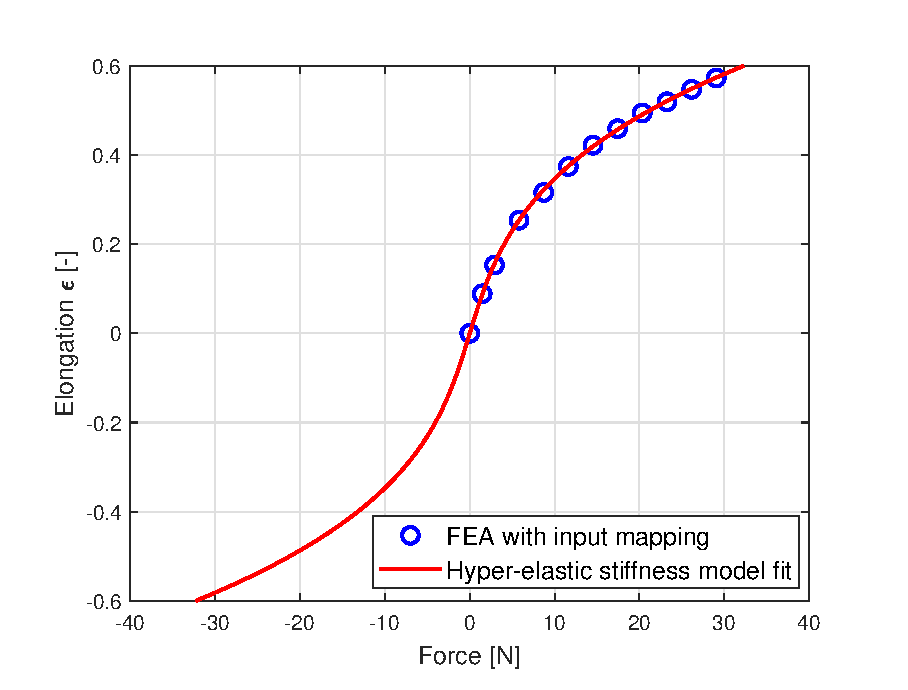
\includegraphics[width=\textwidth]{Figures/Chapter3/mappedforcevselongation.eps}
        \caption{Fitted stiffness model for elongation.}
        \label{fig:pe}
    \end{minipage}\hfill
    \begin{minipage}{0.5\textwidth}
        \centering
        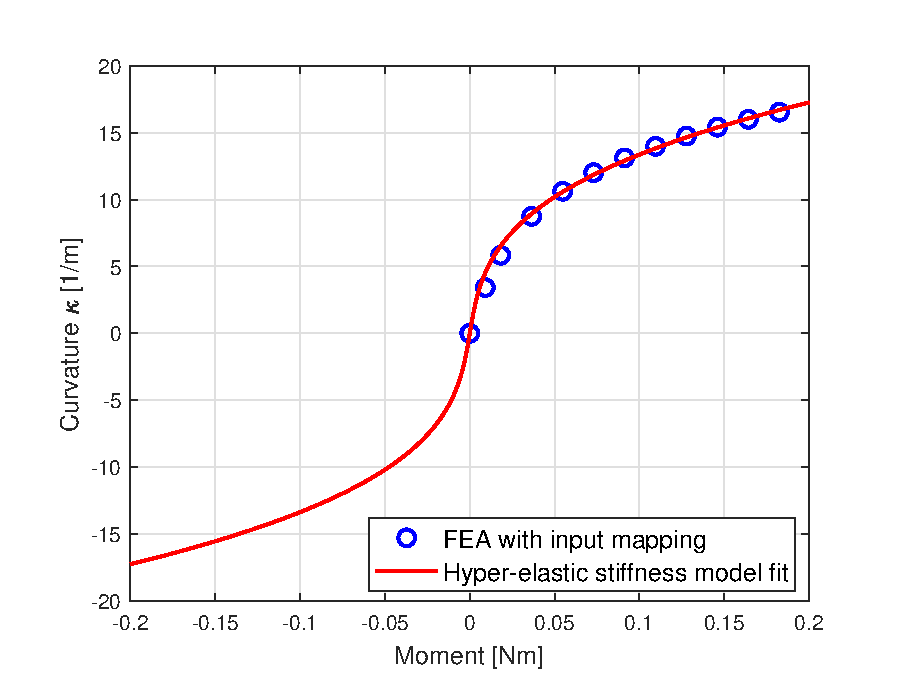
\includegraphics[width=\textwidth]{Figures/Chapter3/mappedmomentvscurvature.eps} 
        \caption{Fitted stiffness model for curvature.}
        \label{fig:pk}
    \end{minipage}
\end{figure}

The determined stiffness allows to develop a non-linear dynamic model formulated as,

\begin{equation}
    M(q)\Ddot{q} + C\dot{q} + K(q)q = u \hspace{10pt} \text{with} \hspace{10pt} u = Hp
    \label{eq:p}
\end{equation}

Were $M$ is the non-linear mass matrix, $C$ a damping matrix, $K$ non-linear stiffness matrix and $H$ a matrix input mapping. Previous meeting it was discussed how this non-linear mass matrix could be obtained. This will be worked out in the next section.


\section{Dynamic model}

This section shows how the non-linear mass matrix is determined. Additionally, results of a free oscillation are presented. 

It is assumed that the total kinetic energy of the actuator can be captured by,

\begin{equation}
    T = \frac{1}{2} \int_0^L V \mathcal{M} V d\sigma
\end{equation}

where $V \in \mathbb{R}^6$ is vector with linear and angular velocities as $[v_x,v_y,v_y,\omega_{x},\omega_{y},\omega_{z}]^\top$. The mass matrix $\mathcal{M} \in \mathbb{R}^{6\times6}$ consists of masses and inertia's $\text{diag}([m_x,m_y,m_z,I_{xx},I_{yy},I_{zz}])$. The planar actuator only has two degrees of freedom, hence we are only interested in $m_z$ and $I_{yy}$. The mass of the actuator is approximated by assuming infinitely thin slices of rectangular shape which are stacked along the length of the actuator. Which gives $m_z$ and $I_{yy}$ as,

\begin{equation}
    m_z = \rho = \frac{m_{total}}{L_0} \hspace{30pt} I_{yy} = \frac{1}{12}\rho w^2
\end{equation}

respectively. Here $m_{total}$ is the mass of the actuator, $L_0$ the undeformed actuator length and $w$ the width of the actuator. The velocity vector can be expresses as,

\begin{equation}
    V = J(\sigma)\dot{q},
\end{equation}

where $J \in \mathbb{R}^{6\times 2}$ is the jacobian and $q \in \mathbb{R}^2$ the vector of modal coordinates. The Jacobian can be determined with \cite{Caasenbrood2020},


\begin{equation}
    J(\sigma) = Ad_g^{-1}(\sigma) \underbrace{\int_0^L Ad_g(\sigma) B_a\Phi(\sigma)d\sigma}_{\Tilde{J}}
    \label{eq:J}
\end{equation}

Without going into further detail, the mass matrix $M(q)$ can be obtained by,

\begin{equation}
    M(q) = \int_0^{\sigma} (\text{Ad}_{g^{-1}}\Tilde{J})^\top \mathcal{M}  \text{Ad}_{g^{-1}}\Tilde{J} d \sigma 
    \label{eq:M}
\end{equation}

Solving Equation (\ref{eq:J}) and (\ref{eq:M}) is done in a Matlab function by rewriting the integral as an ODE. The second order system of (\ref{eq:p}) is rewritten to a first order state-space and becomes,

\begin{equation}
     \begin{bmatrix} \dot{x} \end{bmatrix}   =      \begin{bmatrix} O_2 & I_2 \\ -M^{-1}K(q)  & -M^{-1}D \end{bmatrix}      \begin{bmatrix} x \end{bmatrix}  +      \begin{bmatrix} O_2 \\ M^{-1}H   \end{bmatrix}       \begin{bmatrix} p_1\\ p_2   \end{bmatrix} 
\end{equation}

Simulating the system of for $x_0 = [\epsilon \hspace{2pt} \kappa \hspace{2pt} \dot{\epsilon} \hspace{2pt} \dot{\kappa}]^\top = [0.1 \hspace{2pt} 11 \hspace{2pt} 0 \hspace{2pt} 0]^\top $. No pressure input is given to the system. The system's response is shown in Figure (\ref{fig:sim}).


\begin{figure}[H]
    \centering
    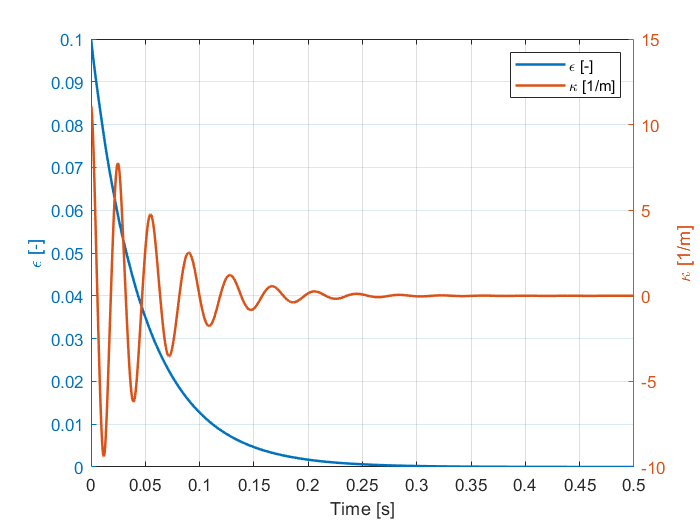
\includegraphics[width = \textwidth]{Figures/ProgresFigures/sim.png}
    \caption{Simulation of the dynamic model}
    \label{fig:sim}
\end{figure}

For this damping parameters it can be seen that the actuator's elongation is critically damped. After 0.25 seconds it reaches it's original length. The actuator will return in its upright position, as the curvature goes to zero as well. Here some periodic swings are observed. The nonlinear stiffness can be seen from the width of the peaks. High curvatures result in narrow peaks, while lower curvatures show wider peaks. Furthermore, it can be seen that the period time regarding the curvature is around 0.03 seconds. Although no experimental data is present, this period time is very small. This indicates that the inertia approximation might not be that good. For now, experimental data is necessary in order to qualitatively compare this dynamic model with the physical actuator's behavior.

\newpage

\section{Revised planning}

I revised the planning, and came with several changes. First of all, the 2-link planar soft robot with gripper might have been too opportunistic when starting this graduation project. Secondly, the situation regarding Corona and distance education contributed to less efficient communication and almost no lab time. Therefore, I have revised the planning as shown in Table (\ref{tab1:projectplanning}). During the meeting I will walk you through the updated planning. Ofcourse, we should agree upon this planning, aswell as the research outcomes and dates. 




\begin{table}[H]
    \centering
    \begin{tabular}{|p{8.1cm}|c|c|} \hline
      \textbf{Description}                        & \textbf{Start}    & \textbf{Finish}    \\ \hline
      Operating planar robot                      & Early Oct         & Mid Oct\\  \hline
      Forward/Inverse Kinematics             & Mid Oct           & Early Nov\\  \hline
      Parameter Estimation in FEM                 & Early Nov         & Mid Dec \\  \hline
      Develop dynamic model                       & Early Dec         & End Jan  \\  \hline
      Controller design (PD,PD+CTC/Jacobian/?)                & Mid Jan           & Early Feb \\  \hline
      Control architecture (interaction  sensors, pumps, Raspberry PI) & Mid Jan  & Mid Feb \\  \hline
      Create home set-up & End Jan  & Early Feb \\  \hline      
      Pressure control (PI-control)            & Early Feb         & Mid/End Feb \\  \hline
      Compare dynamic model (quasi-static)  & Mid Feb           & End Feb/Early March \\  \hline
      Implement PD-controller and perform set-point regulation & Early March & End March \\  \hline
      Modelbased controller design                & Mid March   &  Mid/ End April \\  \hline
      Write thesis                                & Mid March         & Early May \\  \hline
      Oral defence                                & Early May         & Mid May \\ \hline
    \end{tabular}
    \caption{Proposed project planning.}
    \label{tab1:projectplanning}
\end{table}

